\chapter{Design dell'Ontologia}

\section{Classificazione delle Automobili}

In Carpedia, la gerarchia delle automobili (Figura \ref{fig:carpedia-car}) svolge il ruolo di una tassonomia fondamentale per classificare e organizzare vari tipi di veicoli. La gerarchia delle automobili è essenziale per rappresentare e categorizzare i veicoli in base alle loro caratteristiche e ai loro attributi.

Alla radice della gerarchia si trova la classe \texttt{Car}. Questa classe racchiude attributi e proprietà essenziali comuni a tutti i tipi di automobili. Queste proprietà includono:

\begin{itemize}
    \item \texttt{hasKilometers}: Un numero intero positivo che rappresenta il numero di chilometri percorsi da un'auto.
    \item \texttt{hasMaxSpeedKmph}: Un numero intero positivo che indica la velocità massima dell'auto in chilometri all'ora.
    \item \texttt{hasModel}: Una stringa che rappresenta il modello dell'auto.
    \item hasPlate: Una stringa che indica la targa dell'auto.
    \item \texttt{hasPrice}: Un numero intero positivo che indica il prezzo dell'auto.
    \item \texttt{hasSeats}: Un numero intero positivo che rappresenta il numero di posti nell'auto.
    \item \texttt{hasVariant}: Una stringa che descrive la variante o il livello di allestimento dell'auto.
    \item \texttt{hasWeight}: Un numero intero positivo che indica il peso dell'auto.
\end{itemize}

La gerarchia si estende ulteriormente per includere diverse sottoclassi, ognuna delle quali rappresenta un tipo o una categoria specifica di auto. Queste sottoclassi ereditano le proprietà della classe base \texttt{Car} e possono aggiungere eventualmente attributi unici. Le sottoclassi nella nostra ontologia includono:

\begin{itemize}
    \item \texttt{3DoorsCar}: Rappresenta le auto a tre porte.
    \item \texttt{5DoorsCar}: Rappresenta le auto a cinque porte.
    \item \texttt{LuxuryCar}: Rappresenta automobili di lusso di alta gamma.
    \item \texttt{NewlyLicensedCar}: Rappresenta auto adatte a neopatentati.
    \item \texttt{Supercar}: Rappresenta supercar ad alte prestazioni.
\end{itemize}

\begin{figure}[H]
    \caption{Caption: TODO}
    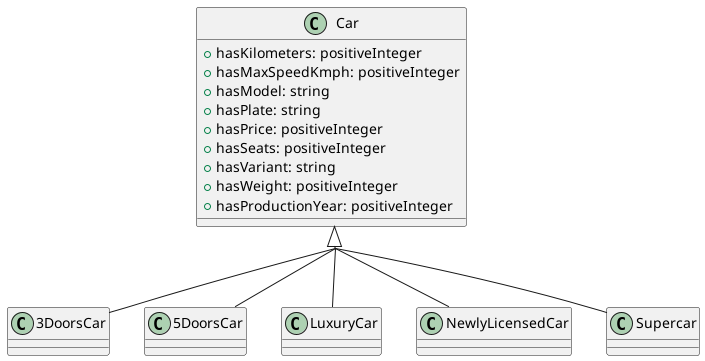
\includegraphics[width=\textwidth]{figures/carpedia-car.png}
    \label{fig:carpedia-car}
\end{figure}

\section{Classificazione dei Componenti}

La gerarchia dei componenti (Figura \ref{fig:carpedia-component}), all'interno di Carpedia, svolge un ruolo centrale nell'organizzazione e nella categorizzazione dei vari componenti e sottosistemi presenti nei sistemi automobilistici. Questa struttura gerarchica consente di rappresentare le intricate relazioni e dipendenze tra diverse parti di un veicolo.

Al centro della nostra gerarchia dei componenti si trova la classe base \texttt{Component}. Questa classe funge da entità fondamentale per tutti i componenti all'interno dell'ontologia. La classe \texttt{Component} definisce una sola proprietà condivisa: Una stringa che rappresenta il numero seriale o l'identificatore associato al componente.

La gerarchia dei componenti si estende per includere diverse sottoclassi, ognuna delle quali rappresenta un tipo o una categoria specifica di componente automobilistico. Queste sottoclassi ereditano la proprietà comune \texttt{hasSerialNumber} dalla classe base \texttt{Component} e possono introdurre attributi aggiuntivi unici per i rispettivi tipi di componente.

\begin{figure}[H]
    \caption{Caption: TODO}
    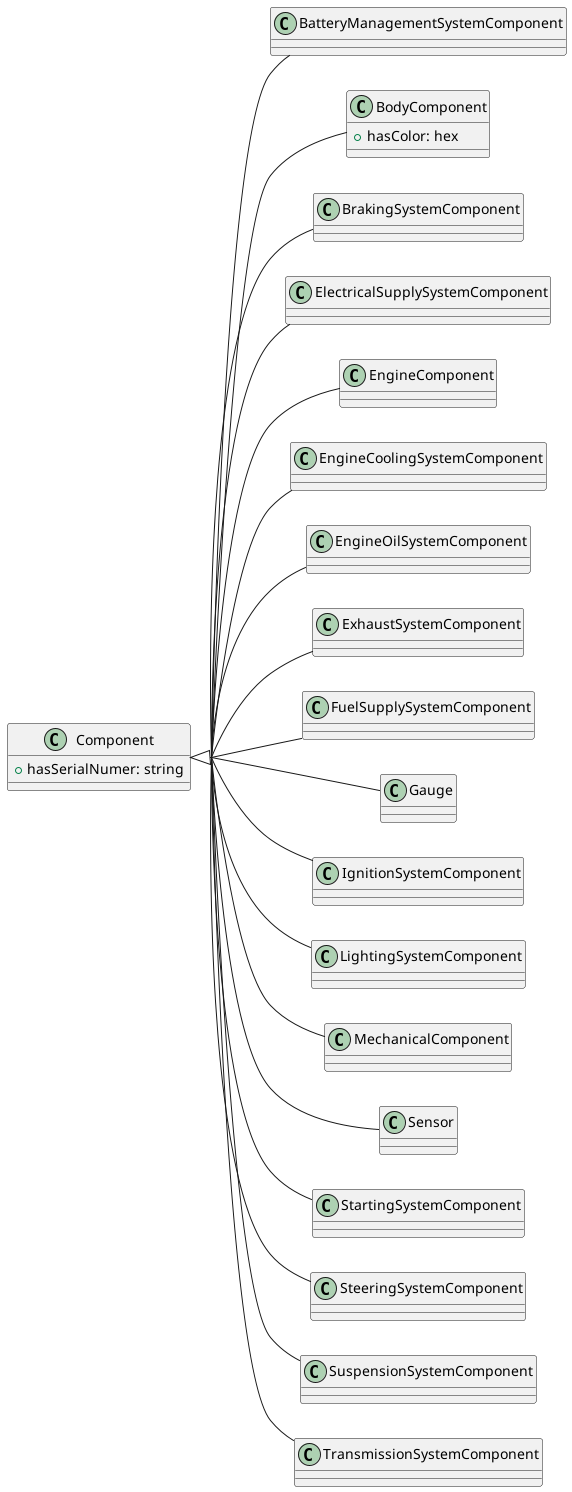
\includegraphics[height=\textheight]{figures/carpedia-component.png}
    \label{fig:carpedia-component}
\end{figure}

\section{Classificazione dei Sistemi}

La gerarchia dei sistemi (Figura \ref{fig:carpedia-system}) è una struttura fondamentale che consente la rappresentazione completa e la classificazione di vari sistemi presenti nei veicoli automobilistici. Questa disposizione gerarchica permette di modellare le relazioni e le dipendenze tra i diversi sistemi e il veicolo.

Al centro della gerarchia dei sistemi si trova la classe base \texttt{System}. Questa classe funge da entità fondamentale per la rappresentazione e la categorizzazione dei vari sistemi all'interno di un veicolo automobilistico. La classe \texttt{System} non definisce attributi specifici, ma invece costituisce la classe genitore per una serie di sottoclassi, ognuna specializzata nella rappresentazione di sistemi automobilistici distinti.

\begin{figure}[H]
    \caption{Caption: TODO}
    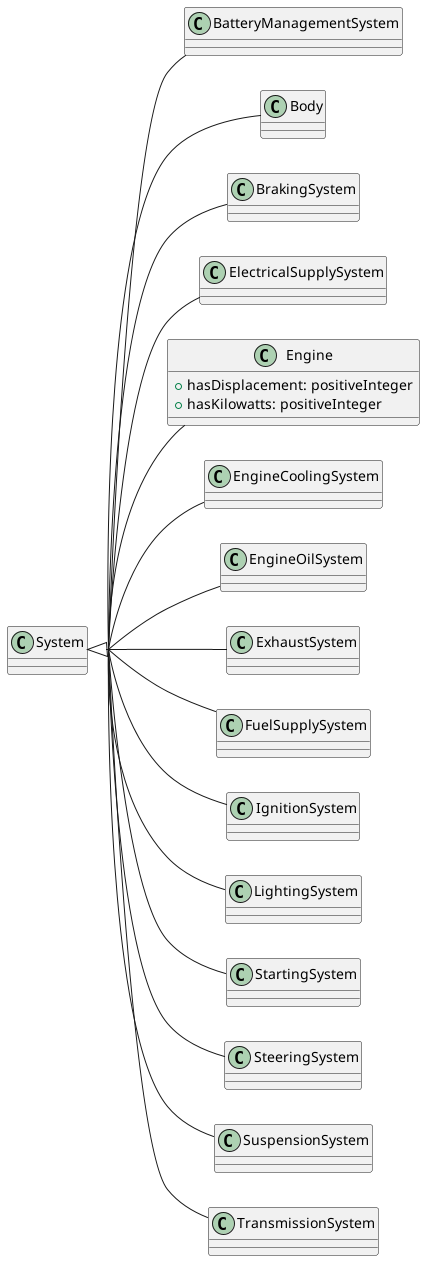
\includegraphics[height=\textheight]{figures/carpedia-system.png}
    \label{fig:carpedia-system}
\end{figure}

\section{Classificazione dei Carburanti}

\begin{figure}[H]
    \caption{Caption: TODO}
    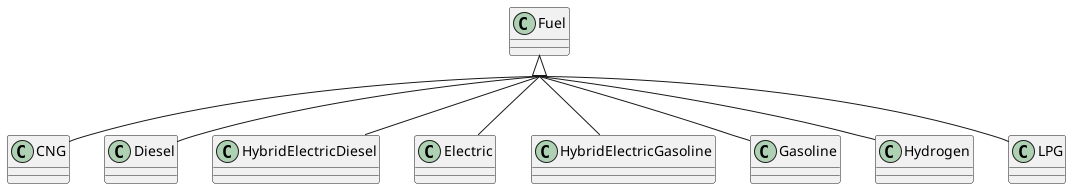
\includegraphics[width=\textwidth]{figures/carpedia-fuel.png}
    \label{fig:carpedia-fuel}
\end{figure}

\section{Classificazione delle Classi di Emissioni}

La gerarchia delle emissioni è un sistema di classificazione cruciale che  consente di rappresentare e categorizzare diverse normative sulle emissioni dei veicoli, concentrandosi in particolare sulle normative sulle emissioni dell'Unione Europea. Questa gerarchia aiuta a modellare l'impatto ambientale e la conformità dei veicoli rispetto alle loro emissioni.

Al radice della gerarchia si trova la classe base \texttt{EuroEmissionClass}. Questa classe funge da fondamento per la rappresentazione delle diverse normative sulle emissioni. Sebbene possa non definire attributi specifici, costituisce la classe principale per una serie di sottoclassi, ognuna delle quali rappresenta una specifica normativa sulle emissioni.

\begin{figure}[H]
    \caption{Caption: TODO}
    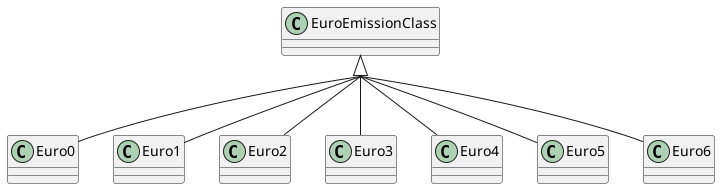
\includegraphics[width=\textwidth]{figures/carpedia-euro-emission.png}
    \label{fig:carpedia-euro-emission}
\end{figure}

\section{Object Properties}

In Carpedia, le \textit{object properties} svolgono un ruolo centrale nell'instaurare relazioni tra le diverse classi. Queste proprietà definiscono come diversi elementi all'interno dell'ontologia sono correlati tra loro, consentendo di modellare associazioni complesse e dipendenze. Il diagramma in Figura \ref{fig:carpedia-object-properties} illustra le principali \textit{object properties} nell'ontologia:

\begin{figure}[H]
    \caption{Caption: TODO}
    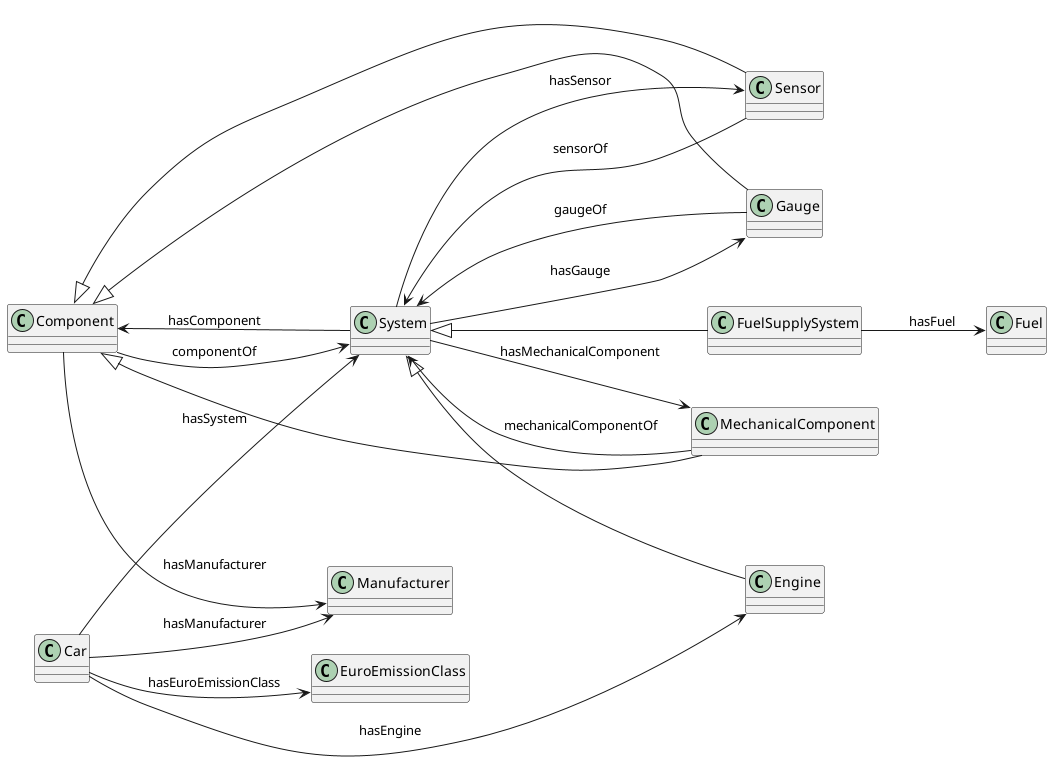
\includegraphics[width=\textwidth]{figures/carpedia-object-properties.png}
    \label{fig:carpedia-object-properties}
\end{figure}

Le \textit{object properties} associate a \texttt{Component} e \texttt{System} sono fondamentali per comprendere come diverse parti di un veicolo automobilistico interagiscono. Queste relazioni sono cruciali per modellare la composizione e la struttura dei veicoli. Di seguito vengono dettagliate queste \textit{object properties}:

\begin{itemize}
    \item \texttt{componentOf}: Questa proprietà stabilisce una connessione tra un \texttt{Component} e un \texttt{System}, indicando che un \texttt{Component} fa parte di un \texttt{System}. Al contrario, la classe \texttt{System} ha la proprietà inversa, \texttt{hasComponent}, che indica che un \texttt{System} può avere più \texttt{Component}. Questa relazione ci consente di rappresentare la struttura gerarchica dei sistemi automobilistici.
    \item \texttt{gaugeOf}: La classe \texttt{Gauge} è correlata a un \texttt{System} mediante questa proprietà, indicando che uno strumento è associato a un particolare sistema. La proprietà inversa, \texttt{hasGauge}, è definita all'interno della classe \texttt{System}, permettendoci di associare strumenti ai sistemi e viceversa.
    \item \texttt{mechanicalComponentOf}: Simile a \texttt{componentOf}, questa proprietà collega \texttt{MechanicalComponent} a \texttt{System} rappresentando la presenza di componenti meccanici all'interno di un sistema. La proprietà inversa, \texttt{hasMechanicalComponent}, è utilizzata all'interno della classe \texttt{System} per denotare l'inclusione di componenti meccanici.
    \item \texttt{sensorOf}: Questa proprietà stabilisce una connessione tra un \texttt{Sensor} e \texttt{System}, indicando che i sensori fanno parte di un sistema. La classe \texttt{System} ha la corrispondente proprietà inversa, \texttt{hasSensor}, per rappresentare l'associazione dei sensori con i sistemi.
\end{itemize}

Oltre alle relazioni legate ai componenti, Carpedia definisce diverse altre \textit{object properties} che catturano vari aspetti del dominio automobilistico:

\begin{itemize}
    \item \texttt{hasEuroEmissionClass}: Questa proprietà collega una macchina alla sua corrispondente classe di emissioni, consentendo di specificare la normativa sulle Emissioni Euro a cui una macchina aderisce. Aiuta a tenere traccia e categorizzare i veicoli in base alle normative sulle emissioni.
    \item \texttt{hasFuel}: La classe \texttt{FuelSupplySystem} è correlata alla classe \texttt{Fuel} utilizzando questa proprietà. Rappresenta il tipo di carburante associato a un sistema di alimentazione, aiutando a caratterizzare il meccanismo di alimentazione del veicolo.
    \item \texttt{hasManufacturer}: Sia le classi \texttt{Car} che \texttt{Component} hanno una relazione con la classe \texttt{Manufacturer} attraverso questa proprietà. Permette di attribuire veicoli e componenti ai rispettivi produttori, facilitando la rintracciabilità e il recupero delle informazioni sul prodotto.
    \item \texttt{hasSystem}: Questa proprietà collega una macchina ai suoi vari sistemi, come il motore, il sistema di frenata e altro ancora.
    \item \texttt{hasEngine}: Specificamente per le automobili, questa proprietà collega una macchina al suo motore.
\end{itemize}
